%! Author = adam
%! Date = 28.02.21

\chapter{Ion Beam Transport and Optics}\label{ch:ion-beam-transport-and-optics}

Once we have accelerated the ions, we want to put them on a path towards a sample (or whatever goal you have in mind with these ions).
The path that they take cane be straight or curved, but regardless the motion is directed a combination of deflectors and lenses.
With the help of EM fields, we can not only focus particles (as is the case with normal lenses), but also accelerate or decelerate particles, as well as direct the particles onto particular paths.
This topic was introduced by Hans Bush in 1926.

\section{Deflection}\label{sec:deflection}
Deflection, as the name suggests, has to do with the directing of the particles as opposed to the accelerating or focusing of particles.
The two types of deflectors we discuss are the electrostatic and electromagnetic deflectors.
For electrostatic deflectors, we refer to those attached to the cyclotron, but the cases made generally hold for other accelerators.
The general idea involves using the Lorentz force, given below. $$ \vec{F} = q(\vec{E} + \vec{v} \times \vec{B}) $$

\subsection{Electrostatic}\label{subsec:electrostatic}

There are two general classes of electrostatic deflectors: devices on which the applied voltage is DC (Direct Current) only, and devices on which the deflecting potential is a sum of instantaneous RF (Radio Frequency) voltage on the dee and the constant DC voltage applied.
Figures of both are given in~\ref{fig:deflectors}.
Before we go into detail about the two, we first consider a simple example.
Consider two plates of opposite charge with an electric field between them.
A positively charged particle entering the area between the plates with motion parallel to the surface of the plates will then experience a pull in the direction of the field (opposite for negatively charged particles), and be deflected with a parabolic path.
The motion of the particle is no longer parallel to the surface of the plates but is then curved.
If the path was in the direction of the field lines (perpendicular to the surface of the plates), then the positively charged particle would experience an acceleration, and for a corresponding deceleration on the path in the direction opposite of the field lines.

\begin{figure}
\begin{subfigure}{0.5\textwidth}
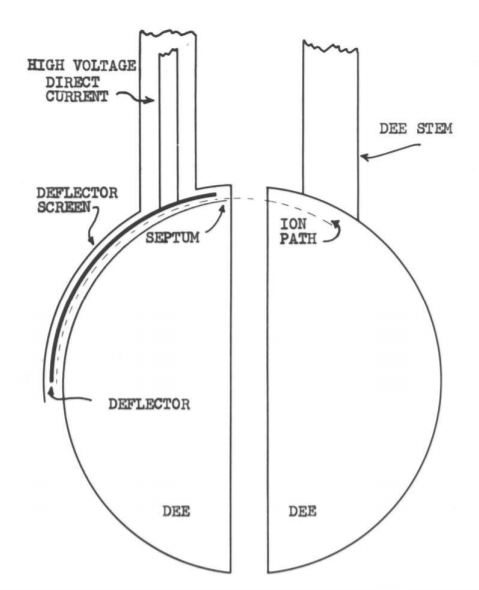
\includegraphics[width=0.9\linewidth, height=5cm]{DCdeflect.png}
\caption{A DC deflector}
\label{fig:DCdeflector}
\end{subfigure}
\begin{subfigure}{0.5\textwidth}
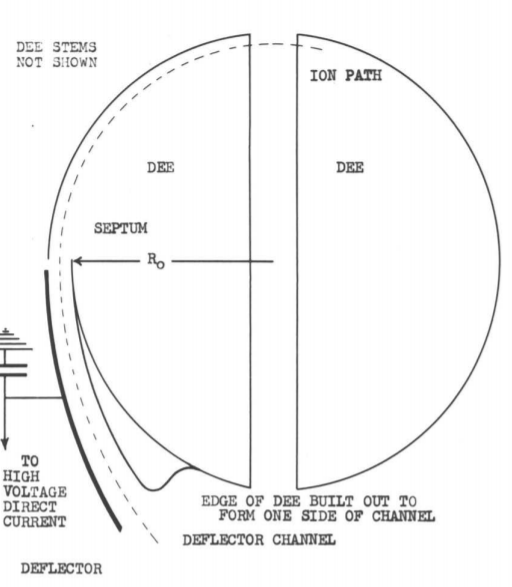
\includegraphics[width=0.9\linewidth, height=5cm]{RFdeflect.png}
\caption{A RF deflector}
\label{fig:RFdeflector}
\end{subfigure}
\caption{Two types of electrostatic deflectors, taken from~\cite{1}}
\label{fig:deflectors}
\end{figure}
The DC deflector, found in Figure~\ref{fig:DCdeflector}, allows complete control over the deflecting potential that is independent of the phase of the circulating ions.
No capacitance is added to the dee system by the deflector.
This is importance since all the power input to the dees will not be lost through the deflector.
The disadvantages of a DC deflector include the fact that incredibly high potentials are required to pull the ions away from the magnetic field which holds them in a circular path (in the case of cyclotrons, but can also be thought of generally).
If one was using an accelerator that is a low voltage (cyclotron, LINAC) then one still would need some shielding gas for the high potential of the DC deflector.
Also, any adjustment of the deflector would be a mechanical one, thus be internal and quite difficult to adjust.
These problems are eliminated by the RF deflector, seen in Figure~\ref{fig:RFdeflector}.
The RF deflector utilizes the high RF potentials existing in the cyclotron, and contains of a strip of metal extending over an arc of 60--90 degrees that forms one side of a deflecting channel.
The channel is the region through which the ions pass and in which the electrostatic field is formed.
What is called the septum is the entrance to the channel, which is a strip of metal that can be quickly tuned via a potential applied to the metal such that the deflector spacing is varied.
This is the important advantage to the RF deflector.

A simpler case is a device called the \textit{steerer}, which consists of a series connection of devices consisting of two charged plates (as discussed in the general case).
The devices are then producing electric field opposite relative to each other such that they take turns deflecting the ions such that an overall change in the particle path.
Depending on the distance between the connection of the two devices, called the drift length $d$, the ion will be deflected by a distance $\Delta a$ compared to the incident.
The end path is still parallel to the initial ion beam.
\subsection{Electromagnetic}\label{subsec:electromagnetic}

In the electromagnetic case, consider a field line similar to our example for the electrostatic case (instead of an E field, we have a B field perpendicular to the 'surface' of two plates).
For ions moving transverse to the field, it will end up in a circular path from the Lorentz force.
If the ion has a velocity component that is not perfectly perpendicular to the magnetic field, it will spiral upwards or downwards in addition to the circular motion.
For high energy particles (high velocity), it is better to use the electromagnetic deflection, as the $\vec{v}$ component of the Lorentz force dominates, and will have a bigger impact on the deflection force on the particle.
There is also what is called the magnetic field steerer as discussed in the electrostatic case.
A device consisting of a 2 magnetic dipole  in the x and y directions.
The ion is then passing through similarly, but this time we have a magnetic field is reversed from transitioning from one device to the next.
The ion is the similarly deflected, but instead of the field line being in the direction of motion in the electrostatic case, it is perpendicular (in this case if the particle is traveling left to right along the surface of this page, the first magnetic field device would produce a $\vec{B}$ field into the page, that would deflect the particle in the downward direction (relative to the writing of this page).
Then the second device would have a magnetic field directed out of the page such that the net effect of both would be a translation of the beam path as before.

\section{Lenses}\label{sec:lenses}
Now lets say we want to focus our ion beams.
Simplest case is a \textit{tube lens}.
This is similar to the combination of a convex and a concave lens in optics.
Not only does deflection occur in this lens, since a voltage is applied across the two tubes, you are also increasing the energy of the ions, since $\Delta \Phi \neq 0$, but rather $ = U$, the voltage applied.
Due to the curvature of the tubes,  similar to the shape of the convex lens, the beam is focused.
A more sophisticated design is the so called \textit{einzel lens} which can be found in Figure \ref{fig:einzel}.
Similar to the tube lens, we are using a combination of three separate tubes (cylindrical or not, just symmetric), where the middle of the three acts as the einzel lens.
This is a charged particle electrostatic lens that focuses without changing the energy of the beam.
The electrostatic potential in the lens is symmetric, so the ions will regain their initial energy on exiting the lens, although the velocity of the outer particles will be altered such that they converge on to the axis.
This causes the outer particles to arrive at the focus intersection slightly later than the ones that travel along a straight path, as they have to travel an extra distance.
The math is as follows:
The equation for the change in radial velocity for a particle if it passes between any pair of cylinders in the lens is $$\Delta v_r = \int \frac{q\vec{E}_r(\vec{r},z)}{mv_z}dz, $$ with $\textbf{z}$ axis passing through the middle of the lens and $r$ being the direction normal to $\textbf{z}$.
If the lens is constructed with cylindrical electrodes, the field is symmetrical around $\textbf{z}$.
The magnitude of the electric field in the radial direction for a particle at a particular radial distance and distance across the gap, is given by $\vec{E}_r(\vec{r},z)$, and $m$ is the mass of the particle passing through the field.
$v_z$ is the velocity of the particle and $q$ the charge.
The integral occurs over the gap between the plates, where the lensing occurs.

\begin{figure}
	\centering
	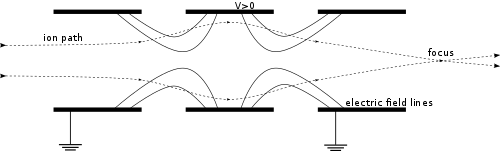
\includegraphics[width=0.9\linewidth, height=5cm]{Einzel_lens_draw.svg.png}
	\caption{Einzel lens configuration. It is important to note that ions traveling near the top or bottom (closer to the cylinders) will have a longer path than those in the middle of the cylinders. This will result in ions being seperated in time, since they are all traveling the same velocity (assuming they had the same initial velocities) as the einzel lens does not accelerate the ions. }
	\label{fig:einzel}
\end{figure}

Another interesting lens is the quadrupole lens.
These are often used in ion trapping, but can also be used in the lens cases.
The mathematics works the same as if you were to use multipole lens, where we include transfer matrices and such.
The general equation for a magnetic field is a combination of terms corresponding to the type of pole you are using.
For example, assume you have a particle traveling in the $z$ direction, and regardless of how many poles you use, your magnetic field is in the $x$ and $y$ directions, i.e., $\vec{v}= (0, 0, v_s)$, $\vec{B} = (B_x, B_y, 0)$.
Then the force acting on the particle is $F = mv_s^2 / R$ where $R$ is the radius of the circular motion of the particle.
We can split up the components of the force in the $x$ direction, perpendicular to the velocity of the particle as $F_x = -qv_sB_y$, and the radius of the motion is given by $1/R(x,y,z) = \frac{q}{p}B_y(x,y,s)$. This term on the RHS dependent on the type of pole you use. So the combination would be:
$$ \frac{q}{p}B_y(x) = \frac{q}{p}\left( B_y(0) + \frac{\partial B_y}{\partial x} x + \frac{1}{2!}\frac{\partial^2 B_y}{\partial x^2} x^2 + \frac{1}{3!}\frac{\partial^3 B_y}{\partial x^3} x^3 + \dots\right) $$  The first term on the RHS is the dipol and the second the quadrapol. These two are called terms of linear ion optics, whereas the next two, the sextupol and oktopul, correspond to non-linear ion optics.
Lens configurations can get as complicated as one wishes, for example the omega lens, or bessel box photon stop.
In order to verify if a lens system will work before the money is spent in building it, it is often recommend to simulate your structure before hand.
Simulation software like \href{https://simion.com/}{SIMION} work well in this.

\section{Selectors}
Let's say you did a handful of focusing lenses and deflectors, and now you have a wide variety of ions with different energies.
You may want to select ions with a particular energy.
In that case you can use what are called velocity selectors.
These can be as complicated as quadrupole magnets, or as simple as a Wien filter.
Basically you introduce a magnetic field and or electric field such that the particles that which have the appropriate (desired) velocity (for Wien filter: $v = \frac{E}{B}$), are passed through the 'filter'.
Those that do not drop off in contact with the filter.

\section{Summary}

\begin{myitemize}
	\item Once a particle is sufficiently accelerated, we can use lens/deflectors to control the beam to a destination using only the Lorentz force
	\item Deflectors can be as simple as a combination of charged plates that translate the ion beam path a distance away from the original path, these devices are called steerers
	\item Lens work similarly to optical lenses, but by using EM fields, examples include the tube lens as well as the einzel lens.
	\item Lenses can not only focus but also accelerate particles.
	\item Electrostatic and Magnetic lenses can also be used to select particles of a certain energy.
    Monochromatic beams can be created using this method of velocity selection (see Wien Filter).
\end{myitemize}